% Options for packages loaded elsewhere
\PassOptionsToPackage{unicode}{hyperref}
\PassOptionsToPackage{hyphens}{url}
%
\documentclass[
  8pt,
  ignorenonframetext,
]{beamer}
\usepackage{pgfpages}
\setbeamertemplate{caption}[numbered]
\setbeamertemplate{caption label separator}{: }
\setbeamercolor{caption name}{fg=normal text.fg}
\beamertemplatenavigationsymbolsempty
% Prevent slide breaks in the middle of a paragraph
\widowpenalties 1 10000
\raggedbottom
\setbeamertemplate{part page}{
  \centering
  \begin{beamercolorbox}[sep=16pt,center]{part title}
    \usebeamerfont{part title}\insertpart\par
  \end{beamercolorbox}
}
\setbeamertemplate{section page}{
  \centering
  \begin{beamercolorbox}[sep=12pt,center]{part title}
    \usebeamerfont{section title}\insertsection\par
  \end{beamercolorbox}
}
\setbeamertemplate{subsection page}{
  \centering
  \begin{beamercolorbox}[sep=8pt,center]{part title}
    \usebeamerfont{subsection title}\insertsubsection\par
  \end{beamercolorbox}
}
\AtBeginPart{
  \frame{\partpage}
}
\AtBeginSection{
  \ifbibliography
  \else
    \frame{\sectionpage}
  \fi
}
\AtBeginSubsection{
  \frame{\subsectionpage}
}
\usepackage{amsmath,amssymb}
\usepackage{lmodern}
\usepackage{iftex}
\ifPDFTeX
  \usepackage[T1]{fontenc}
  \usepackage[utf8]{inputenc}
  \usepackage{textcomp} % provide euro and other symbols
\else % if luatex or xetex
  \usepackage{unicode-math}
  \defaultfontfeatures{Scale=MatchLowercase}
  \defaultfontfeatures[\rmfamily]{Ligatures=TeX,Scale=1}
\fi
% Use upquote if available, for straight quotes in verbatim environments
\IfFileExists{upquote.sty}{\usepackage{upquote}}{}
\IfFileExists{microtype.sty}{% use microtype if available
  \usepackage[]{microtype}
  \UseMicrotypeSet[protrusion]{basicmath} % disable protrusion for tt fonts
}{}
\makeatletter
\@ifundefined{KOMAClassName}{% if non-KOMA class
  \IfFileExists{parskip.sty}{%
    \usepackage{parskip}
  }{% else
    \setlength{\parindent}{0pt}
    \setlength{\parskip}{6pt plus 2pt minus 1pt}}
}{% if KOMA class
  \KOMAoptions{parskip=half}}
\makeatother
\usepackage{xcolor}
\newif\ifbibliography
\setlength{\emergencystretch}{3em} % prevent overfull lines
\providecommand{\tightlist}{%
  \setlength{\itemsep}{0pt}\setlength{\parskip}{0pt}}
\setcounter{secnumdepth}{-\maxdimen} % remove section numbering
\newlength{\cslhangindent}
\setlength{\cslhangindent}{1.5em}
\newlength{\csllabelwidth}
\setlength{\csllabelwidth}{3em}
\newlength{\cslentryspacingunit} % times entry-spacing
\setlength{\cslentryspacingunit}{\parskip}
\newenvironment{CSLReferences}[2] % #1 hanging-ident, #2 entry spacing
 {% don't indent paragraphs
  \setlength{\parindent}{0pt}
  % turn on hanging indent if param 1 is 1
  \ifodd #1
  \let\oldpar\par
  \def\par{\hangindent=\cslhangindent\oldpar}
  \fi
  % set entry spacing
  \setlength{\parskip}{#2\cslentryspacingunit}
 }%
 {}
\usepackage{calc}
\newcommand{\CSLBlock}[1]{#1\hfill\break}
\newcommand{\CSLLeftMargin}[1]{\parbox[t]{\csllabelwidth}{#1}}
\newcommand{\CSLRightInline}[1]{\parbox[t]{\linewidth - \csllabelwidth}{#1}\break}
\newcommand{\CSLIndent}[1]{\hspace{\cslhangindent}#1}
% type setting
% ------------------------------------------------------------------------------
\usepackage[german]{babel}     

% fonts
% ------------------------------------------------------------------------------
\usefonttheme{professionalfonts}

% slide title and horizontal line
% ------------------------------------------------------------------------------
\setbeamertemplate{frametitle}{%
    \vskip-30pt \color{black}\large%
    \begin{minipage}[b][23pt]{120mm}%
    \flushleft\insertframetitle%
    \end{minipage}%
}

\setbeamertemplate{headline}										
{
\vskip10pt\hfill\hspace{3.5mm} 										 
\vskip15pt\color{black}\rule{\textwidth}{0.4pt} 					 
}

% slide number
% ---------------------------------------------------------------
\setbeamertemplate{navigation symbols}{}
\setbeamertemplate{footline}
{
\vskip5pt
\vskip2pt
\makebox[123mm]{\hspace{7.5mm}
\hfill Psychologische Forschungsmethoden $\vert$ 
\copyright $ $ 2023 Dirk Ostwald CC BY-SA 4.0 $\vert$ 
Folie \insertframenumber}
\vskip4pt
}

% block color scheme
% ------------------------------------------------------------------------------
% colors
\definecolor{white}{RGB}{255,255,255}
\definecolor{grey}{RGB}{235,235,235}
\definecolor{lightgrey}{RGB}{245,245,245}
\definecolor{LightBlue}{RGB}{220,220,255}
\definecolor{darkblue}{RGB}{51, 51, 153}

% definitions and theorems
\setbeamercolor{block title}{fg = black, bg = grey}
\setbeamercolor{block body}{fg = black, bg = lightgrey}

% general line spacing 
% ------------------------------------------------------------------------------
\linespread{1.3}

% local line spacing
% ------------------------------------------------------------------------------
\usepackage{setspace}

% colors
% -----------------------------------------------------------------------------
\usepackage{color}

% justified text
% ------------------------------------------------------------------------------
\usepackage{ragged2e}
\usepackage{etoolbox}
\apptocmd{\frame}{}{\justifying}{}

% bullet point lists
% -----------------------------------------------------------------------------
\setbeamertemplate{itemize item}[circle]
\setbeamertemplate{itemize subitem}[circle]
\setbeamertemplate{itemize subsubitem}[circle]
\setbeamercolor{itemize item}{fg = black}
\setbeamercolor{itemize subitem}{fg = black}
\setbeamercolor{itemize subsubitem}{fg = black}
\setbeamercolor{enumerate item}{fg = black}
\setbeamercolor{enumerate subitem}{fg = black}
\setbeamercolor{enumerate subsubitem}{fg = black}
\setbeamerfont{itemize/enumerate body}{}
\setbeamerfont{itemize/enumerate subbody}{size = \normalsize}
\setbeamerfont{itemize/enumerate subsubbody}{size = \normalsize}

% color links
% ------------------------------------------------------------------------------
\usepackage{hyperref}
\definecolor{urls}{RGB}{204,0,0}
\hypersetup{colorlinks, citecolor = darkblue, urlcolor = urls}


% additional math commands
% ------------------------------------------------------------------------------
\usepackage{bm}                                         % bold math symbols
\newcommand{\niton}{\not\owns}

% text highlighting
% ------------------------------------------------------------------------------
\usepackage{soul}
\makeatletter
\let\HL\hl
\renewcommand\hl{%
  \let\set@color\beamerorig@set@color
  \let\reset@color\beamerorig@reset@color
  \HL}
\makeatother

% equation highlighting
% -----------------------------------------------------------------------------
\newcommand{\highlight}[2][yellow]{\mathchoice%
  {\colorbox{#1}{$\displaystyle#2$}}%
  {\colorbox{#1}{$\textstyle#2$}}%
  {\colorbox{#1}{$\scriptstyle#2$}}%
  {\colorbox{#1}{$\scriptscriptstyle#2$}}}%

% additional mathematical operators
% ------------------------------------------------------------------------------
\DeclareMathOperator*{\argmax}{arg\,max}
\DeclareMathOperator*{\argmin}{arg\,min}

\ifLuaTeX
  \usepackage{selnolig}  % disable illegal ligatures
\fi
\IfFileExists{bookmark.sty}{\usepackage{bookmark}}{\usepackage{hyperref}}
\IfFileExists{xurl.sty}{\usepackage{xurl}}{} % add URL line breaks if available
\urlstyle{same} % disable monospaced font for URLs
\hypersetup{
  hidelinks,
  pdfcreator={LaTeX via pandoc}}

\author{}
\date{\vspace{-2.5em}}

\begin{document}

\begin{frame}[plain]{}
\protect\hypertarget{section}{}
\center

\begin{center}
\includegraphics[width=0.2\linewidth]{6_Abbildungen/pfm_6_otto} \end{center}

\vspace{2mm}

\Large

Psychologische Forschungsmethoden \vspace{6mm}

\normalsize

BSc Philosophie-Neurowissenschaften-Kognition WiSe 2022/23

BSc Psychologie WiSe 2022/23

\large
\vspace{6mm}

Prof.~Dr.~Dirk Ostwald
\end{frame}

\begin{frame}{}
\protect\hypertarget{section-1}{}
\vspace{1mm}

\textcolor{darkblue}{Vorläufige Vorlesungsübersicht}

\small
\center
\footnotesize
\renewcommand{\arraystretch}{1.1}
\begin{tabular}{lll}
Datum        & Einheit                       & Thema                                                           \\\hline
13.10.2022   & Formalia                      & (0) Formalia                                            \\
13.10.2022   & Psychologische Wissenschaft   & (1) Wissenschaft                                        \\
20.10.2022   & Psychologische Wissenschaft   & (2) Grundlagenorientierte psychologische Wissenschaft   \\
27.10.2022   & Psychologische Wissenschaft   & (2) Anwendungsorientierte psychologische Wissenschaft   \\
03.11.2022   & Psychologische Wissenschaft   & (3) Psychologische Daten                                \\
10.11.2022   & Messtheorie                   & (4) Einführung Messtheorie                              \\
17.11.2022   & Messtheorie                   & (5) Relationen                                          \\
24.11.2022   & Messtheorie                   & (6) Grundprobleme der Messtheorie                       \\
01.12.2022   & Messtheorie                   & (7) Skalenarten                                         \\
08.12.2022   & Messtheorie                   & (8) Ordinalmessung                                      \\
15.12.2022   & Messtheorie                   & (9) Extensivmessung                                     \\
05.01.2023   & Messtheorie                   & (10) Differenzmessung                                   \\
12.01.2023   & Messtheorie                   & (11) Bedeutsamkeit                                      \\
19.01.2023   & Messtheorie                   & (12) Psychophysik                                       \\
26.01.2023   & Messtheorie                   & (13) Likertskalen                                        \\\hline
29.03.2023   & Klausurtermin                 & 12:00 – 13:00 Uhr, G16 – H5                             \\
Juli 2023    & Klausurwiederholungstermin    &
\end{tabular}
\end{frame}

\begin{frame}[plain]{}
\protect\hypertarget{section-2}{}
\vfill
\center
\huge

\textcolor{black}{(6) Grundprobleme der Messtheorie} \vfill
\end{frame}

\begin{frame}{}
\protect\hypertarget{section-3}{}
\vfill
\Large
\setstretch{3}

Grundidee des Messens

Homomorphismen und Skalen

Repräsentation, Eindeutigkeit, Bedeutsamkeit

Selbstkontrollfragen \vfill
\end{frame}

\begin{frame}{}
\protect\hypertarget{section-4}{}
\vfill
\Large
\setstretch{3}

\textbf{Grundidee des Messens}

Homomorphismen und Skalen

Repräsentation, Eindeutigkeit, Bedeutsamkeit

Selbstkontrollfragen \vfill
\end{frame}

\begin{frame}{Grundidee des Messens}
\protect\hypertarget{grundidee-des-messens}{}
\begin{center}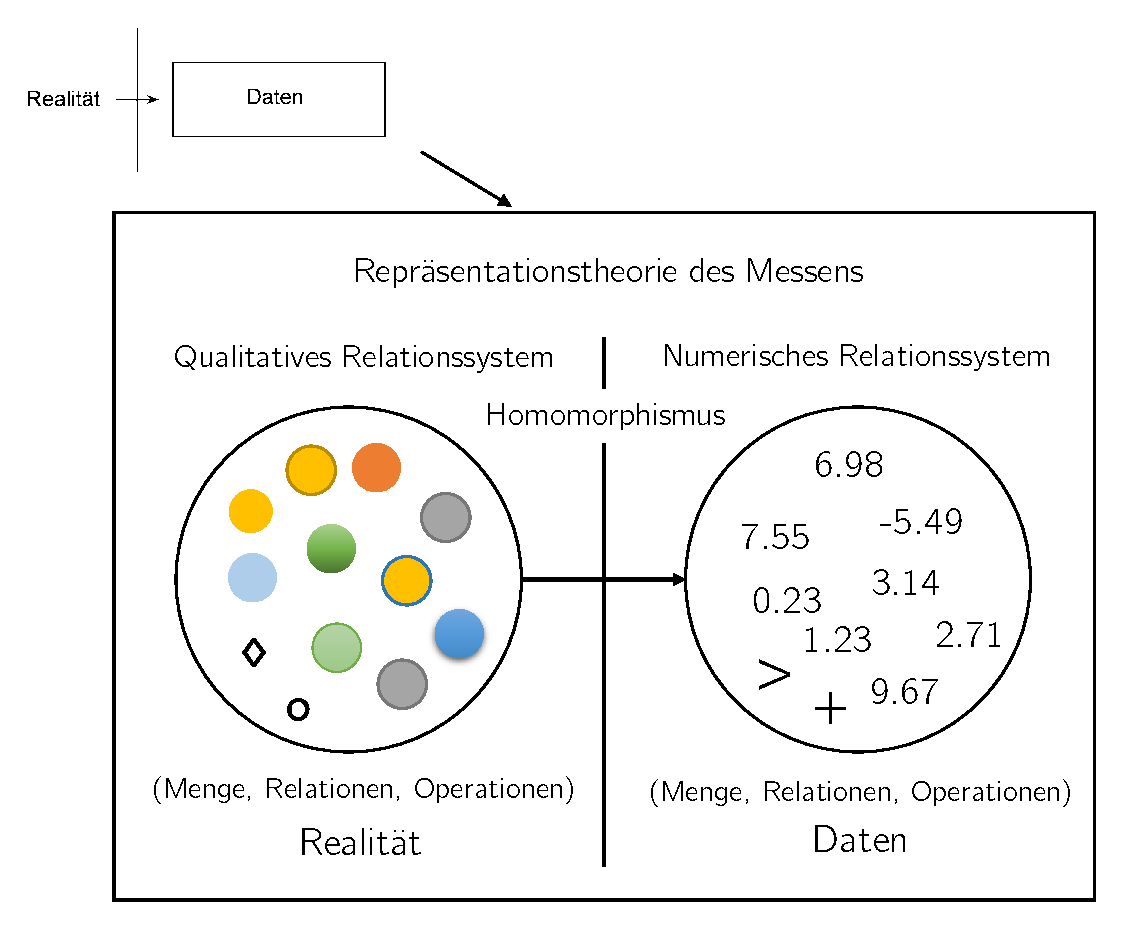
\includegraphics[width=0.7\linewidth]{6_Abbildungen/pfm_6_messtheorie} \end{center}

\footnotesize
\center

Die Grundidee des Messens ist es, Eigenschaften von Objekten Zahlen so
zuzuweisen, dass die Relationen der Eigenschaften der Objekte sowie
Operationen mit Objekteigenschaften im Bereich der Zahlen erhalten
bleiben.
\end{frame}

\begin{frame}{Grundidee des Messens}
\protect\hypertarget{grundidee-des-messens-1}{}
\small

\textcolor{darkblue}{Beispiel (1) Messen von Entscheidungsoptionspräferenzen}

\footnotesize
\justifying

Messen der Entscheidungsoptionspräferenzen eines Agenten bedeutet, den
Entscheidungsoptionen Zahlen so zuzuordnen, dass die qualitative
Relation ``Entscheidungsoption \(m\) wird präferiert über
Entscheidungsoption \(n\)'' in der Realität im Bereich der Zahlen
erhalten bleibt.

Sei \(M\) die Menge von Entscheidungsoptionen und sei \(R\) die
Entscheidungsoptionspräferenzrelation, d.h. für \(m,n \in M\) gelte
\begin{equation}
m \mbox{ wird präferiert über } n \Leftrightarrow (m,n) \in R .
\end{equation} Dann möchte man bei der Messung von
Entscheidungsoptionspräferenzen \(m\) und \(n\) so mithilfe einer
Funktion \(f\) Zahlen zuordnen, dass gilt \begin{equation}
m \mbox{ wird präferiert über } n \Leftrightarrow (m,n) \in R \Leftrightarrow f(m) > f(n).
\end{equation} Eine solche Funktion heißt dann \emph{Nutzenfunktion
(utility function)}.

Das Messen von Entscheidungsoptionspräferenzen wird in der Folge unser
Beispiel für den Begriff der \emph{Ordinalmessung} und den zugehörigen
Begriff der \emph{Ordinalskala} sein.
\end{frame}

\begin{frame}{Grundidee des Messens}
\protect\hypertarget{grundidee-des-messens-2}{}
\small

\textcolor{darkblue}{Beispiel (2) Messen der Masse von Objekten}
\footnotesize

Messen der Masse eines Objektes bedeutet, den Objekten Zahlen so
zuzuordnen, dass die qualitative Relation ``Objekt \(m\) ist schwerer
als Objekt \(n\)'' in der Realität im Bereich der Zahlen erhalten
bleibt. Weiterhin möchte man beim Messen der Masse eines Objektes auch
sicherstellen, dass der Messprozess additiv ist, d.h. dass die Masse der
physischen Kombination zweier Objekte der Summation der Massen der
einzelnen Objekte entspricht.

Sei \(M\) die Menge von Objekten, sei \(R\) die
Gewichtsvergleichrelation, d.h. für \(m,n \in M\) gelte \begin{equation}
m \mbox{ ist schwerer als } n \Leftrightarrow (m,n) \in R
\end{equation} und \(\circ\) sei die Operation des physischen
Kombinierens zweier Objekte, d.h. für \(m,n \in M\) gelte
\begin{equation}
m \mbox{ wird kombiniert mit } n \Leftrightarrow m \circ n.
\end{equation} Dann möchte man bei der Messung der Masse von Objekten
\(m\) und \(n\) so mit Hilfe einer Funktion \(f\) Zahlen zuordnen, dass
gilt \begin{equation}
m \mbox{ ist schwerer als } n \Leftrightarrow (m,n) \in R \Leftrightarrow f(m) > f(n)
\end{equation} und \begin{equation}
f(m \mbox{ wird kombiniert mit } n) \Leftrightarrow f(m \circ n) = f(m) + f(n).
\end{equation} Eine solche Funktion heißt \emph{Waage}.

Das Messen der Masse von Objekten wird in der Folge unser Beispiel für
den Begriff der \emph{Extensivmessung} und den zugehörigen Begriff der
\emph{Verhältnisskala} sein.
\end{frame}

\begin{frame}{}
\protect\hypertarget{section-5}{}
\vfill
\Large
\setstretch{3}

Grundidee des Messens

\textbf{Homomorphismen und Skalen}

Repräsentation, Eindeutigkeit, Bedeutsamkeit

Selbstkontrollfragen \vfill
\end{frame}

\begin{frame}{Homomorphismen und Skalen}
\protect\hypertarget{homomorphismen-und-skalen}{}
\small
\begin{definition}[Homomorphismus]
\justifying
$\mathcal{M} := (M,R_1,...,R_p, \circ_1, ...,\circ_q)$ und
$\mathcal{N} := (N,\tilde{R}_1,...,\tilde{R}_p, \tilde{\circ}_1, ...,\tilde{\circ}_q)$
seien zwei Relationssysteme gleichen Typs. Dann heißt eine Funktion $f : M \to N$
ein \textit{Homomorphismus von $\mathcal{M}$ nach $\mathcal{N}$}, wenn $f$ folgende
Eigenschaften hat:
\begin{itemize}
\item[(1)] Für alle $i = 1,...,p$ und alle $m_1,...,m_{r_i} \in M$ gilt
\begin{equation}
(m_1,...,m_{r_i}) \in R_i \Leftrightarrow (f(m_1),...,f(m_{r_i})) \in \tilde{R}_i.
\end{equation}
\item[(2)] Für alle $i = 1,...,q$ und alle $m,n\in M$ gilt
\begin{equation}
f(m \circ_i n) = f(m) \tilde{\circ}_i f(n).
\end{equation}
\end{itemize}
Wenn zwischen zwei Relationssystemen $\mathcal{M}$ und $\mathcal{N}$ gleichen Typs
ein Homomorphismus existiert, dann heißen $\mathcal{M}$ und $\mathcal{N}$ \textit{homomorph}.
\end{definition}

\begin{definition}[Isomorphismus]
Ein injektiver Homomorphismus heißt \textit{Isomorphismus}. Wenn zwischen zwei
Relationssystemen $\mathcal{M}$ und $\mathcal{N}$ gleichen Typs ein Isomorphismus
existiert, dann heißen $\mathcal{M}$ und $\mathcal{N}$ \textit{isomorph}.
\end{definition}
\end{frame}

\begin{frame}{Homomorphismen und Skalen}
\protect\hypertarget{homomorphismen-und-skalen-1}{}
\footnotesize
\vspace{1mm}

Bemerkungen \vspace{-1mm}

\begin{itemize}
\tightlist
\item
  \justifying Die Definition eines Homomorphismus basiert auf der
  Existenz zweier Relationssysteme gleichen Typs.
\item
  In der Messtheorie ist \(\mathcal{M}\) meist ein qualitatives
  Relationssystem und \(\mathcal{N}\) ein numerisches Relationssystem.
\item
  Eigenschaft (1) besagt, dass wenn ein \(r_i\)-Tupel von Elementen in
  \(M\) ein Element der \(i\)ten Relation \(R_i\) auf \(M\) ist, dann
  soll das \(r_i\)-Tupel der durch \(f\) transformierten Elemente ein
  Element der \(i\)ten Relation \(\tilde{R}_i\) auf \(N\) sein und
  umgekehrt.
\item
  Eigenschaft (2) besagt, dass für \(i = 1,...,q\) die durch \(f\)
  transfomierte \(i\)te Verknüpfung zweier Elemente aus \(M\) auf \(M\)
  gleich der \(i\)ten Verknüpfung der durch \(f\) transfomierten
  Elemente aus \(M\) auf \(N\) sein soll.
\item
  Für einen Isomorphismus gilt neben den Eigenschaften (1) und (2) noch,
  dass \(f\) injektiv ist, also dass für \(m,n\in M\) gilt, dass
  \begin{equation}
  m \neq n \Rightarrow f(m) \neq f(n) \mbox{ bzw. } f(m) = f(n) \Rightarrow m = n.
  \end{equation}
\item
  Die Definition eines Homomorphismus ist für endlich viele Relationen
  und Operationen auf Mengen formuliert.
\item
  Im Fall des Messen von Entscheidungsoptionspräferenzen betrachtet man
  \(\mathcal{M} = (M,R)\) und \(\mathcal{N} = (\mathbb{R},>)\) und fragt
  mit \(p := 1, r_1 := 2\) und \(q:=0\) dementsprechend nach einer
  Funktion \(f\), für die gilt \begin{equation}
  (m,n) \in R \Leftrightarrow f(m) > f(n).
  \end{equation}
\item
  Im Fall des Messen der Masse von Objekten betrachtet man
  \(\mathcal{M} = (M,R,\circ)\) und \(\mathcal{N} = (\mathbb{R},>,+)\)
  und fragt mit \(p := 1,r_1 := 2\) und \(q:=1\) dementsprechend nach
  einer Funktion \(f\), für die gilt \begin{equation}
  (m,n) \in R \Leftrightarrow f(m) > f(n)
  \mbox{ und }
  f(m \circ n) = f(m) + f(n).
  \end{equation}
\end{itemize}
\end{frame}

\begin{frame}{Homomorphismen und Skalen}
\protect\hypertarget{homomorphismen-und-skalen-2}{}
\setstretch{1.2}
\small

Beispiel

\footnotesize

Es sei \(\mathcal{M} := (M,R)\) das \((2,0)\) Relationssystem mit
\(M := \{a,b,c,d\}\) und \begin{equation}
R := \{(a,b), (b,c), (a,c), (a,d), (b,d), (c,d)\}
\end{equation} Weiterhin sei \(\mathcal{N} := (\mathbb{R},>)\) ein
numerisches Relationssystem.

Dann ist \begin{equation}
f : M \to \mathbb{R}, m \mapsto f(m) \mbox{ mit }
f(a) := 4, f(b) := 3, f(c) := 2, f(d) := 1
\end{equation} ein Homomorphismus von \(\mathcal{M}\) nach
\(\mathcal{N}\), weil \begin{align}
\begin{split}
(a,b) \in R \Leftrightarrow a \diamond b  & \Leftrightarrow f(a) > f(b) \Leftrightarrow 4 > 3 \Leftrightarrow (4,3) \in\, > \\
(b,c) \in R \Leftrightarrow b \diamond c  & \Leftrightarrow f(b) > f(c) \Leftrightarrow 3 > 2 \Leftrightarrow (3,2) \in\, > \\
(a,c) \in R \Leftrightarrow a \diamond c  & \Leftrightarrow f(a) > f(c) \Leftrightarrow 4 > 2 \Leftrightarrow (4,2) \in\, > \\
(a,d) \in R \Leftrightarrow a \diamond d  & \Leftrightarrow f(a) > f(d) \Leftrightarrow 4 > 1 \Leftrightarrow (4,1) \in\, > \\
(b,d) \in R \Leftrightarrow b \diamond d  & \Leftrightarrow f(b) > f(d) \Leftrightarrow 3 > 1 \Leftrightarrow (3,1) \in\, > \\
(c,d) \in R \Leftrightarrow c \diamond d  & \Leftrightarrow f(c) > f(d) \Leftrightarrow 2 > 1 \Leftrightarrow (2,1) \in\, > \\
\end{split}
\end{align} Für die hier definierten Relationssysteme \(\mathcal{M}\)
und \(\mathcal{M}\) existiert also ein Homomorphismus.

Es ist dementsprechend leicht einzusehen, dass auch \begin{equation}
g : M \to \mathbb{R}, m \mapsto g(m) \mbox{ mit }
g(a) := 10, g(b) := 4, g(c) := 2, g(d) := 0
\end{equation} ein Homomorphismus von \(\mathcal{M}\) nach
\(\mathcal{N}\) ist. Für die hier definierten Relationssysteme
\(\mathcal{M}\) und \(\mathcal{M}\) existiert also sogar mehr als nur
ein Homomorphismus.
\end{frame}

\begin{frame}{Homomorphismen und Skalen}
\protect\hypertarget{homomorphismen-und-skalen-3}{}
\small
\begin{definition}[Skala]
\justifying
$\mathcal{M}$ sei ein qualitatives Relationssystem mit Menge $M$, $\mathcal{N}$ sei
ein numerisches Relationssystem und
\begin{equation}
\mathcal{H}(\mathcal{M}, \mathcal{N}) := \lbrace h : M \to \mathbb{R} | h \mbox{ ist ein Homomorphismus von } \mathcal{M} \mbox{ nach } \mathcal{N} \rbrace
\end{equation}
sei die Menge aller Homomorphismen von $\mathcal{M}$ nach  $\mathcal{N}$. Dann
heißt für eine Funktion $f : M \to \mathbb{R}$ das Tripel $(\mathcal{M}, \mathcal{N},f)$
\textit{Skala}, wenn $f\in \mathcal{H}(\mathcal{M},\mathcal{N})$.
\end{definition}

Bemerkungen

\begin{itemize}
\tightlist
\item
  Die hier gewählte Definition entspricht der Definition der
  \emph{numerischen Skala} in Roberts (1984).
\item
  Wenn \(\mathcal{H}(\mathcal{M}, \mathcal{N}) = \emptyset\), dann
  existiert kein Homomorphismus von \(\mathcal{M}\) nach
  \(\mathcal{N}\).
\item
  Wenn \(|\mathcal{H}(\mathcal{M}, \mathcal{N})| > 1\) , dann existieren
  mehr als ein Homomorphismus von \(\mathcal{M}\) nach \(\mathcal{N}\).
\item
  Der Begriff ``Skala'' wird manchmal auch nur nur für einen
  Homomorphimus verwendet.
\item
  In der Psychologie wird der Begriff ``Skala'' auch oft als Synonym für
  ``Fragebogen'' verwendet.
\end{itemize}
\end{frame}

\begin{frame}{}
\protect\hypertarget{section-6}{}
\vfill
\Large
\setstretch{3}

Grundidee des Messens

Homomorphismen und Skalen

\textbf{Repräsentation, Eindeutigkeit, Bedeutsamkeit}

Selbstkontrollfragen \vfill
\end{frame}

\begin{frame}{Repräsentation, Eindeutigkeit, Bedeutsamkeit}
\protect\hypertarget{repruxe4sentation-eindeutigkeit-bedeutsamkeit}{}
\small
\begin{definition}[Repräsentationsproblem der Messtheorie]
\justifying
Gegeben seien ein qualitatives Relationssystem $\mathcal{M}$ und ein numerisches 
Relationssystem $\mathcal{N}$. Dann besteht das \textit{Repräsentationsproblem der Messtheorie} 
darin, notwendige und hinreichende Eigenschaften von $\mathcal{M}$ für die Existenz eines
Homomorphismus von $\mathcal{M}$ nach $\mathcal{N}$ anzugeben.
\end{definition}

\footnotesize

Bemerkungen

\begin{itemize}
\tightlist
\item
  \justifying Für ein gegebenes numerisches Relationssystem
  \(\mathcal{N}\) fragt man also, wie ein qualitatives Relationssystem
  \(\mathcal{M}\) beschaffen sein muss, damit ein Homomorphismus von
  \(\mathcal{M}\) nach \(\mathcal{N}\) existiert.
\item
  Messtheoretische Theoreme, die besagen, dass bestimmte Eigenschaften
  von \(\mathcal{M}\) für die Existenz eines Homomorphismus von
  \(\mathcal{M}\) nach \(\mathcal{N}\) notwendig und hinreichend sind,
  heißen \textit{Repräsentationstheoreme}.
\item
  Im Idealfall ist der Beweis eines Repräsentationstheorems
  \textit{konstruktiv}, d.h., neben dem Beweis der bloßen Existenz des
  Homomorphismus gibt der Beweis auch die funktionale Form des
  Homomorphismus an und definiert damit den Messvorgang.
\item
  Die notwendigen und hinreichenden Eigenschaften von \(\mathcal{M}\)
  für die Existenz eines Homomorphismus von \(\mathcal{M}\) nach
  \(\mathcal{N}\) werden traditionell auch \emph{Axiome} von
  \(\mathcal{M}\) genannt.
\item
  In den Einheiten (8) Ordinalmessung, (9) Extensivmessung und (10)
  Differenzmessung addressieren wir die jeweiligen
  Repräsentationsprobleme.
\end{itemize}
\end{frame}

\begin{frame}{Repräsentation, Eindeutigkeit, Bedeutsamkeit}
\protect\hypertarget{repruxe4sentation-eindeutigkeit-bedeutsamkeit-1}{}
\setstretch{1.2}
\small

\textcolor{darkblue}{Notwendige und hinreichende Eigenschaften}
\footnotesize

Wir erinnern an die Bedeutung \emph{notwendiger und hinreichender
Eigenschaften (Bedingungen)}.

Eigenschaften \(B\) sind eine notwendige Bedingung für eine Aussage
\(K\), wenn sie zwingend erfüllt sein müssen, wenn \(K\) erfüllt ist.
Man schreibt dafür \(K \Rightarrow B\), ``aus \(K\) folgt \(B\)''.
Gemahlene Bohnen sind eine notwendige Bedingung beim Kochen von Kaffee,
d.h. wenn Kaffee gekocht wird, existieren gemahlene Bohnen. Hinreichend
für das Kochen von Kaffee sind gemahlene Bohnen aber nicht, es braucht
ja z.B. auch noch Wasser und Hitze. Bei der Frage nach Nullstellen einer
Funktion \(f : \mathbb{R} \to \mathbb{R}\) ist eine notwendige Bedingung
für das Vorliegen einer Extremstelle in \(x\), dass \(f'(x) = 0\). Wenn
also \(f\) an der Stelle \(x\) eine Extremstelle hat, dann gilt
\(f'(x) = 0\). Hinreichend für eine Extremstelle von \(f\) in \(x\) ist
\(f'(x) = 0\) allerdings nicht, denn es gilt auch \(f'(x) = 0\) in
Sattelpunkten. Im Kontext der messtheoretischen Repräsentation sind
notwendige Eigenschaften von \(\mathcal{M}\) solche Eigenschaften von
\(\mathcal{M}\), die aus der Existenz eines Homomorphismus von
\(\mathcal{M}\) nach \(\mathcal{N}\) folgen.

Eigenschaften \(B\) sind eine hinreichende Bedingung für eine Aussage
\(K\), wenn aus \(B\) zwingend folgt, dass \(K\) erfüllt ist. Man
schreibt dafür \(B \Rightarrow K\), ``aus \(B\) folgt \(K\)''.
Nassfutter zu fressen ist eine hinreichende Bedingung für die Sättigung
des Katers, d.h. wenn der Kater Nassfutter gefressen hat, ist er satt.
Allerdings ist Nassfutter zu fressen keine notwendige Bedingung für die
Sättigung des Katers, denn auch wenn der Kater Trockenfutter gefressen
hat, ist er satt. Bei der Frage nach Nullstellen einer Funktion
\(f : \mathbb{R} \to \mathbb{R}\) sind hinreichende Bedingungen für das
Vorliegen einer Extremstelle in \(x\), dass \(f'(x) = 0\) und
\(f''(x) \neq 0\). Aus \(f'(x) = 0\) und \(f''(x) \neq 0\) folgt
zwingend, dass \(f\) in \(x\) eine Extremstelle hat. Im Kontext der
messtheoretischen Repräsentation sind hinreichende Eigenschaften von
\(\mathcal{M}\) solche Eigenschaften von \(\mathcal{M}\), aus denen die
Existenz eines Homomorphismus von \(\mathcal{M}\) nach \(\mathcal{N}\)
folgen.

Hinreichende und notwendige Eigenschaften \(B\) von \(\mathcal{M}\) für
die Existenz \(K\) eines Homomorphismus sind also ein Minmalset an
Eigenschaften von \(\mathcal{M}\), die für die Existenz eines
Homomorphismus genügen, so dass gilt \begin{equation}
B \Rightarrow K \mbox{ und } K \Rightarrow B \mbox{, also } B \Leftrightarrow K.
\end{equation}
\end{frame}

\begin{frame}{Repräsentation, Eindeutigkeit, Bedeutsamkeit}
\protect\hypertarget{repruxe4sentation-eindeutigkeit-bedeutsamkeit-2}{}
\small
\begin{definition}[Eindeutigkeitsproblem der Messtheorie]
\justifying
Gegeben seien ein qualitatives Relationssystem $\mathcal{M}$, ein numerisches 
Relationssystem $\mathcal{N}$ und ein Homomorphismus $f$ von $\mathcal{M}$ nach $\mathcal{N}$.
Dann besteht das \textit{Eindeutigkeitsproblem der Messtheorie} darin, zu bestimmen, 
ob dieser Homomorphismus der einzige Homomorphismus ist, der zwischen $\mathcal{M}$ 
und $\mathcal{N}$ existiert.
\end{definition}

\footnotesize

Bemerkungen

\begin{itemize}
\tightlist
\item
  \justifying Die Antworten auf Eindeutigkeitsprobleme legen die
  sogenannten \emph{Skalenarten} fest.
\item
  Die Antworten auf Eindeutigkeitsprobleme legen die Grundlage für den
  Begriff der \emph{Bedeutsamkeit}.
\item
  In Einheit (7) Skalenarten befassen wir uns mit dem
  Eindeutigkeitsproblem der Messtheorie.
\end{itemize}
\end{frame}

\begin{frame}{Repräsentation, Eindeutigkeit, Bedeutsamkeit}
\protect\hypertarget{repruxe4sentation-eindeutigkeit-bedeutsamkeit-3}{}
\small
\begin{definition}[Bedeutsamkeit]
\justifying
$\mathcal{M}$ sei ein qualitatives Relationssystem und $\mathcal{N}$ sei ein
numerisches Relationssystem. Dann heißt eine Aussage bezüglich $\mathcal{M}$ und 
$\mathcal{N}$ \textit{bedeutsam}, wenn ihr Wahrheitsgehalt unverändert bleibt, wenn eine
beliebige Skala $(\mathcal{M},\mathcal{N},f)$ durch eine andere Skala
$(\mathcal{M}, \mathcal{N},g)$ ersetzt wird.
\end{definition}

\footnotesize

Bemerkungen

\begin{itemize}
\tightlist
\item
  \justifying Mithilfe der Theorie der Skalenarten kann der Begriff der
  Bedeutsamkeit klarer mithilfe des Begriffs der \emph{zulässigen
  Skalentransformationen} formuliert werden, welchen wir in Einheit (7)
  Skalenarten einführen.
\item
  Der Begriff der Bedeutsamkeit wird manchmal herangezogen, um zu
  argumentieren, dass bestimmte Datenanalysen bei bestimmten Daten
  ``erlaubt'' und andere ``nicht erlaubt sind''. Wir werden diese
  Aspekte in den Einheit (11) Bedeutsamkeit und (12) Likertskalen näher
  beleuchten und kritisch diskutieren.
\item
  Zum Einstieg geben wir im Folgenden zwei Beispiele für intuitiv
  bedeutsame und nicht bedeutsame Aussagen.
\end{itemize}
\end{frame}

\begin{frame}{Repräsentation, Eindeutigkeit, Bedeutsamkeit}
\protect\hypertarget{repruxe4sentation-eindeutigkeit-bedeutsamkeit-4}{}
\small

\textcolor{darkblue}{Beispiele (1) Bedeutsame Aussagen beim Messen der Masse von Objekten}

\footnotesize

Die Aussage ``Objekt \(m\) ist doppelt so schwer wie Objekt \(n\)'' ist
intuitiv bedeutsam, da unabhängig davon, ob in Gramm, Kilogramm (1 kg =
1000 g), oder angloamerikanischen Pfund (1 lb = 0.453 kg) gemessen wird,
die Aussage wahr bleibt.

Seien zum Beispiel den Objekten \(m\) und \(n\) durch die Gramm-Skala
die Gewichte 400 g und 200 g zugeordnet. Dann gilt \begin{equation}
\frac{\mbox{Gewicht von } m}{\mbox{Gewicht von } n} = 2
\rightarrow
\frac{400 \mbox{ g}}{200 \mbox{ g}} = 2
\rightarrow
\frac{0.4 \mbox{ kg}}{0.2 \mbox{ kg}} = 2
\rightarrow
\frac{0.88 \mbox{ lb}}{0.44 \mbox{ lb}} = 2.
\end{equation} \vspace{2mm}

\small

\textcolor{darkblue}{Beispiel (2) Nicht bedeutsame Aussagen beim Messen der Temperatur von Objekten}
\footnotesize

Die Aussage ``Objekt \(m\) ist doppelt so warm wie Objekt \(n\)'' ist
intuitiv nicht bedeutsam, da abhängig davon, ob in Grad Celsius
(T\(_{\mbox{\tiny C}}\)), Fahrenheit (T\(_{\mbox{\tiny F}}\) =
\(\frac{9}{5}\) T\(_{\mbox{\tiny C}}\) + 32), oder Kelvin
(T\(_{\mbox{\tiny K}}\) = T\(_{\mbox{\tiny C}}\) + 275.15) gemessen
wird, die Aussage falsch wird.

Seien zum Beispiel den Objekten \(m\) und \(n\) durch die Celsius-Skala
die Temperaturen 40°C und 20°C zugeordnet. Dann gilt \begin{equation}
\frac{\mbox{Temperatur von } m}{\mbox{Temperatur von } n} = 2
\rightarrow
\frac{40^{\circ} \mbox{C}}{20^{\circ} \mbox{C}} = 2
\rightarrow
\frac{104^{\circ} \mbox{ F}}{68^{\circ} \mbox{ F}} = 1.52 \neq 2
\rightarrow
\frac{313.15\mbox{ K}}{293.15\mbox{ K}} = 1.06 \neq 2.
\end{equation} Das Messen von Temperatur von Objekten wird in der Folge
unser Arbeitsbeispiel für den Begriff der \emph{Differenzmessung} und
dem zugehörigen Begriff der \emph{Intervallskala} sein.
\end{frame}

\begin{frame}{}
\protect\hypertarget{section-7}{}
\vfill
\Large
\setstretch{3}

Grundidee des Messens

Homomorphismen und Skalen

Repräsentation, Eindeutigkeit, Bedeutsamkeit

\textbf{Selbstkontrollfragen} \vfill
\end{frame}

\begin{frame}{Selbstkontrollfragen}
\protect\hypertarget{selbstkontrollfragen}{}
\footnotesize
\setstretch{2}

\begin{enumerate}
\tightlist
\item
  Erläutern Sie die Grundidee des Messens.
\item
  Erläutern Sie das Messen von Entscheidungsoptionspräferenzen.
\item
  Erläutern Sie das Messen der Masse von Objekten.
\item
  Geben Sie die Definition eines Homomorphismus wieder.
\item
  Geben Sie die Definition eines Isomorphismus wieder.
\item
  Geben Sie die Definition einer Skala wieder.
\item
  Definieren Sie das Repräsentationsproblem der Messtheorie.
\item
  Erläutern Sie die Begriffe der notwendigen und hinreichenden
  Eigenschaften eines qualitativen Relationssystems für die Existenz
  eine Homomorphismus.
\item
  Definieren Sie das Eindeutigkeitsproblem der Messtheorie.
\item
  Definieren den messtheoretischen Begriff der Bedeutsamkeit.
\item
  Warum ist die Aussage ``Objekt \(m\) ist doppelt so schwer wie Objekt
  \(n\)'' intuitiv bedeutsam, die Aussage ``Objekt \(m\) ist doppelt so
  warm wie Objekt \(n\)'' dagegehn intuitiv nicht bedeutsam?
\end{enumerate}
\end{frame}

\begin{frame}{Referenzen}
\protect\hypertarget{referenzen}{}
\footnotesize

\hypertarget{refs}{}
\begin{CSLReferences}{1}{0}
\leavevmode\vadjust pre{\hypertarget{ref-roberts_1984}{}}%
Roberts, Fred S. 1984. \emph{Measurement Theory with Applications to
Decisionmaking, Utility, and the Social Sciences}. Encyclopedia of
Mathematics and Its Applications ; {Section}, {Mathematics} and the
Social Sciences, v. 7. Cambridge {[}Cambridgeshire{]} ; New York, NY,
USA: Cambridge University Press.

\end{CSLReferences}
\end{frame}

\end{document}
